\begingroup
\centering
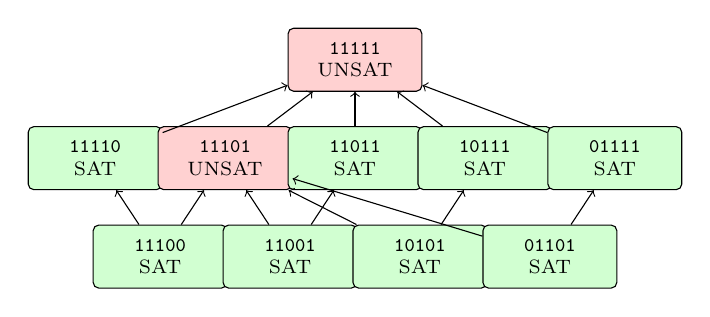
\begin{tikzpicture}[x=1.65cm,y=1.25cm]
\tikzstyle{frontiernode}=[draw, rounded corners=2pt, minimum width=1.7cm, minimum height=0.8cm, align=center, font=\scriptsize]
\node[frontiernode, fill=green!18] (case_11100) at (-1.50,0.00) {\texttt{11100}\\SAT};
\node[frontiernode, fill=green!18] (case_11001) at (-0.50,0.00) {\texttt{11001}\\SAT};
\node[frontiernode, fill=green!18] (case_10101) at (0.50,0.00) {\texttt{10101}\\SAT};
\node[frontiernode, fill=green!18] (case_01101) at (1.50,0.00) {\texttt{01101}\\SAT};
\node[frontiernode, fill=green!18] (case_11110) at (-2.00,1.00) {\texttt{11110}\\SAT};
\node[frontiernode, fill=red!18] (case_11101) at (-1.00,1.00) {\texttt{11101}\\UNSAT};
\node[frontiernode, fill=green!18] (case_11011) at (0.00,1.00) {\texttt{11011}\\SAT};
\node[frontiernode, fill=green!18] (case_10111) at (1.00,1.00) {\texttt{10111}\\SAT};
\node[frontiernode, fill=green!18] (case_01111) at (2.00,1.00) {\texttt{01111}\\SAT};
\node[frontiernode, fill=red!18] (case_11111) at (0.00,2.00) {\texttt{11111}\\UNSAT};
\draw[->, thin] (case_11100) -- (case_11110);
\draw[->, thin] (case_11100) -- (case_11101);
\draw[->, thin] (case_11110) -- (case_11111);
\draw[->, thin] (case_11001) -- (case_11101);
\draw[->, thin] (case_11001) -- (case_11011);
\draw[->, thin] (case_10101) -- (case_11101);
\draw[->, thin] (case_10101) -- (case_10111);
\draw[->, thin] (case_01101) -- (case_11101);
\draw[->, thin] (case_01101) -- (case_01111);
\draw[->, thin] (case_11101) -- (case_11111);
\draw[->, thin] (case_11011) -- (case_11111);
\draw[->, thin] (case_10111) -- (case_11111);
\draw[->, thin] (case_01111) -- (case_11111);
\end{tikzpicture}
\par\medskip
\scriptsize Boundary slice: unsatisfiable cases and their immediate solved predecessors in the subset poset.
\endgroup
